\documentclass[12pt]{article}

\usepackage[utf8]{inputenc}
\usepackage[brazil]{babel}
\usepackage[a4paper,left=3cm, right=2cm,top=3cm, bottom=2cm]{geometry}
\usepackage{amsmath}
\usepackage{graphicx}
\usepackage{float}
\usepackage{authblk}
\usepackage{fancyhdr}
\usepackage{xcolor}

\title{\textbf{Monitoria MAT1202 - Álgebra Linear 2 \\Apostila Notas de Aula }}

\author[]{\textbf{Matheus Nogueira}}

\date{}
\pagestyle{fancy}
\fancyhf{}
\lhead{{\small \textcolor{gray}{Apostila Monitoria MAT1202}}}
\renewcommand{\headrulewidth}{0pt}
\fancyfoot[C]{\thepage}
\begin{document}
	\maketitle
	\begin{abstract}
		Este documento consiste nas notas de aula da monitoria de MAT1202. Este material foi produzido com base em minhas anotações do curso de Álgebra Linear 2 do semestre 20.2 e do livro \textit{Álgebra Linear e suas aplicações}, de \textit{Gilbert Strang}. Qualquer dúvida, favor entrar em contato \textit{matnogueira@gmail.com}
	\end{abstract}
	\tableofcontents
	\pagebreak
	\section{Sistemas Lineares e Eliminação Gaussiana}
	\subsection{Sistemas Lineares e Notação Matricial}
	
	Nosso foco é estudar sistemas de equações da forma $Ax=b$, onde $A$ é a matriz com os termos que acompanham as variáveis (incógnitas), $x$ é o vetor coluna com as incógnitas e $b$ é o vetor coluna com os termos independentes.\\
	
	\textbf{Exemplo:} Seja o seguinte sistema de equações...
	
	\begin{align*}
		x+2y+3&=2\\-x+y-z&=-3\\2x+y-z&=0
	\end{align*}
	
	Escrevê-lo em forma matricial é definir as seguinte matriz e vetores:
	\begin{equation*}
		A=
		\begin{bmatrix}
			1 & 2 & 3\\
			-1 & 1 & -1\\
			2 & 1 & -1
		\end{bmatrix} \mbox{, } 
		x=
		\begin{bmatrix}
			x\\ y\\z
		\end{bmatrix} \mbox{ e } 
		b=
		\begin{bmatrix}
			2 \\ -3\\0
		\end{bmatrix}
	\end{equation*}
	
	Não é difícil perceber que a multiplicação representada por $Ax$ resulta exatamente no sistema linear inicial.
	
	\subsection{Solução de um Sistema Linear}
	
	Nossa estratégia para calcular a solução de um sistema de equações lineares será a \textbf{Eliminação Gaussiana}. 
	
	Este método consiste em realizar operações na matriz do sistema $Ax=b$, chamadas \textit{operações elementares}, para chegar a um \textit{sistema triangular}. Ao ser obtido este sistema, basta realizar uma série de substituições retroativas para chegar à solução.\\
	
	\textbf{Definição:} Matrizes Triangulares
	
	Uma matriz é triangular - superior ou inferior - se todas as entradas abaixo ou acima, respectivamente, da diagonal principal são nulas. A matriz $A$ abaixo é triangular superior, enquanto que $B$ é triangular inferior.
	
	\begin{equation*}
		A=
		\begin{bmatrix}
			1 & 2 & 3\\
			0 & 1 & -1\\
			0 & 0 & -1
		\end{bmatrix} \mbox{, } 
		B=
		\begin{bmatrix}
			1 & 0 &0\\
			-1 & 1 & 0\\
			2 & 1 & -1
		\end{bmatrix}
	\end{equation*}
	
	São 3 os possíveis tipos de solução de um sistema linear:
	\begin{enumerate}
		\item Exatamente 1 solução
		\item Infinitas Soluções
		\item Não há solução
	\end{enumerate}
	
	\textbf{Observação:} lembrem-se que, para verificar qual das opções acima é a o caso da matriz a ser estudada, podemos olhar para o \textit{determinante} da matriz. Se seu valor for zero, o sistema possui infinitas soluções ou nenhuma solução. Se for diferente de zero, uma solução.
	
	\subsubsection{Operações Elementares}
	
	\textbf{Definição:}
	dado um sistema linear $Ax=b$, são 3 as operações elementares que não alteram a solução do sistema.
	\begin{enumerate}
		\item Permutação de linhas ($L_i\leftrightarrow L_j$)
		\item Multiplicação de linha por escalar ($L_i\rightarrow L_i \cdot k,k \neq 0$)
		\item Somar um múltiplo de uma linha a outra linha ($L_i \rightarrow L_i+k\cdot L_j$)
	\end{enumerate}
	
	\subsubsection{Matrizes das operações elementares}
	
	Veremos que cada uma das 3 operações elementares descritas pode ser representada por meio de matrizes da seguinte forma:\\
	
	Se queremos realizar a operação elementar $e$ sobre a matriz $A$, devemos realizar a multiplicação $E\cdot A$, onde $E$ é a matriz que representa a operação elementar $e$. \\
	
	Vejamos as como montar as matrizes para as mesmas 3 operações já apresentadas. Por facilidade, usaremos matrizes $3x3$, pois o raciocínio para outras dimensões é o mesmo. Começamos sempre com a matriz identidade e:
	\begin{enumerate}
		\item Permutação de linhas ($L_i\leftrightarrow L_j$):\\ basta permutar as linhas da matriz identidade de acordo com as linhas a serem permutadas na matriz A
		\item Multiplicação de linha por escalar ($L_i\rightarrow L_i \cdot k,k \neq 0$):\\ multiplicamos a linha correspondente da matriz identidade pelo escalar em questão.
		\item Somar um múltiplo de uma linha a outra linha ($L_i \rightarrow L_i+k\cdot L_j$):\\ colocamos na entrada $i,j$ da matriz identidade o valor de $k$ com o devido sinal.
	\end{enumerate}
	
	\begin{align}
		L_2\leftrightarrow L_3 \implies &
		\begin{bmatrix}
			1 & 0 &0\\
			0 & 1 & 0\\
			0 & 0 & 1
		\end{bmatrix} \leftrightarrow 
		\begin{bmatrix}
			1 & 0 &0\\
			0 & 0 & 1\\
			0 & 1 & 0
		\end{bmatrix}=E\\
		L_2\rightarrow L_2 \cdot k\implies &
		\begin{bmatrix}
			1 & 0 &0\\
			0 & 1 & 0\\
			0 & 0 & 1
		\end{bmatrix} \leftrightarrow 
		\begin{bmatrix}
			1 & 0 &0\\
			0 & k\cdot 1 & 0\\
			0 & 0 & 1
		\end{bmatrix}=E\\
		L_3 \rightarrow L_3-2\cdot L_1 \implies &
		\begin{bmatrix}
			1 & 0 &0\\
			0 & 1 & 0\\
			0 & 0 & 1
		\end{bmatrix} \leftrightarrow 
		\begin{bmatrix}
			1 & 0 &0\\
			0 & 1 & 0\\
			-2 & 0 & 1
		\end{bmatrix}=E
	\end{align}\\
	
	Ao final da \textit{Eliminação Gaussiana}, depois de serem realizadas todas as devidas \textit{operações elementares}, a matriz obtida estará na forma \textbf{escalonada}, isto é:
	\begin{enumerate}
		\item Se existem linhas nulas elas devem ser as últimas da matriz.
		\item Em quaisquer duas linhas sucessivas não nulas, o pivô (primeiro elemento não nulo) da linha inferior deve estar mais à direita que o da linha superior.
		\item Abaixo do pivô todas as entradas são nulas.
	\end{enumerate}
	
	\subsection{Exemplo}
	
	Calculemos a solução do seguinte sistema, mostrando as matrizes das operações elementares.
	
	\begin{align*}
		2x+y+z&=5\\4x-6y&=2\\-2x+7y+2z&=9
	\end{align*}\\
	
	Em forma matricial o sistema é: \\
	
	\begin{equation*}
		\begin{bmatrix}
			2 & 1 & 1\\
			4 & -6 & 0\\
			-2 & 7 & 2
		\end{bmatrix} \cdot
		\begin{bmatrix}
			x\\ y\\z
		\end{bmatrix} =
		\begin{bmatrix}
			5 \\ -2\\9
		\end{bmatrix}
	\end{equation*}
	
	
	Seja a matriz aumentada a ser escalonada a seguir: 
	\begin{equation*}
		\begin{bmatrix}
			2 & 1 & 1 & 5\\
			4 & -6 & 0 & -2\\
			-2 & 7 & 2 & 9
		\end{bmatrix}
	\end{equation*}
	
	Comecemos as operações elementares para chegar à matriz escalonada. A cada operação, indicaremos a matriz $E$ correspondente.
	
	\begin{equation*}
		L_2 \rightarrow L_2 -2L_1 \mbox{ sendo } 
		E_1=\begin{bmatrix}
			1 & 0 &0\\
			-2 & 1 & 0\\
			0 & 0 & 1
		\end{bmatrix}\\
	\end{equation*}
	Nosso sistema fica...
	\begin{equation*}
		\begin{bmatrix}
			2 & 1 & 1 & 5\\
			0 & -8 & -2 & -12\\
			-2 & 7 & 2 & 9
		\end{bmatrix}
	\end{equation*}\\
	
	
	\begin{equation*}
		L_3 \rightarrow L_3 +L_1 \mbox{ sendo } 
		E_2=\begin{bmatrix}
			1 & 0 &0\\
			0 & 1 & 0\\
			1 & 0 & 1
		\end{bmatrix}\\
	\end{equation*}
	Nosso sistema fica...
	\begin{equation*}
		\begin{bmatrix}
			2 & 1 & 1 & 5\\
			0 & -8 & -2 & -12\\
			0 & 8 & 3 & 14
		\end{bmatrix}
	\end{equation*}
	
	
	\begin{equation*}
		L_3 \rightarrow L_3 +L_2 \mbox{ sendo } 
		E_3=\begin{bmatrix}
			1 & 0 &0\\
			0 & 1 & 0\\
			0 & 1 & 1
		\end{bmatrix}\\
	\end{equation*}
	Nosso sistema fica...
	\begin{equation*}
		\begin{bmatrix}
			2 & 1 & 1 & 5\\
			0 & -8 & -2 & -12\\
			0 & 0 & 1 & 2
		\end{bmatrix}
	\end{equation*}
	
	Chegamos à matriz escalonada. Agora basta realizar algumas substituições retroativas para calcularmos a solução.
	
	Lendo e substituindo o sistema de baixo para cima temos:
	
	\begin{align*}
		z&=2 \\
		-8y-2(2)&=-12 \rightarrow y=1 \\
		2x+1+2&=5 \rightarrow x=1	
	\end{align*}
	
	Note que chegamos a uma solução única, o que faz sentido pois $\det(A)=-16\neq0$
	
	Utilizando as matrizes das operações elementares, chegaríamos na mesma matriz escalonada:
	
	\begin{align*}
		E_3\cdot E_2 \cdot E_1 \cdot A &\mbox{ , onde A é a matriz aumentada} \\
		\begin{bmatrix}
			1 & 0 &0\\
			0 & 1 & 0\\
			0 & 1 & 1
		\end{bmatrix}\cdot
		\begin{bmatrix}
			1 & 0 &0\\
			0 & 1 & 0\\
			1 & 0 & 1
		\end{bmatrix} \cdot
		\begin{bmatrix}
			1 & 0 &0\\
			-2 & 1 & 0\\
			0 & 0 & 1
		\end{bmatrix} \cdot&
		\begin{bmatrix}
			2 & 1 & 1 & 5\\
			4 & -6 & 0 & -2\\
			-2 & 7 & 2 & 9
		\end{bmatrix} = 
		\begin{bmatrix}
			2 & 1 & 1 & 5\\
			0 & -8 & -2 & -12\\
			0 & 0 & 1 & 2
		\end{bmatrix}
	\end{align*}
	
	\subsection{Conclusão}
	Com este material sabemos como encontrar a solução de um sistema linear utilizando a Eliminação Gaussiana e as operações Elementares, com suas respectivas matrizes. O próximo assunto a ser abordado será \textbf{Fatoração LU}.
	
	\newpage
	
	
	\section{Fatoração A=LU}
	
	\subsection{Sem permutação de linhas}
	
	No capítulo anterior vimos, ou relembramos,  como resolver um sistema linear utilizando o processo da Eliminação Gaussiana por meio, principalmente, de operações elementares e suas matrizes. Neste capítulo continuaremos estudando sistemas lineares do tipo $Ax=b$ e apresentaremos uma maneira de fatorar a matriz $A$, escrevendo-a como $A=LU$.\\
	
	Dito isso, já podemos definir a matriz $A$ como a matriz de coeficientes do nosso sistema linear, ou seja, exatamente a mesma matriz $A$ do capítulo anterior. Nosso sistema linear é:\\
	\begin{equation*}
		\begin{bmatrix}
			a_{11} & a_{12} & a_{13}\\
			a_{21} & a_{22} & a_{23}\\
			a_{31} & a_{32} & a_{33}
		\end{bmatrix} \cdot
		\begin{bmatrix}
			x\\ y\\z
		\end{bmatrix}=
		\begin{bmatrix}
			b_{11} \\ b_{21} \\ b_{31}
		\end{bmatrix} \mbox{ logo, } \newline
		A=\begin{bmatrix}
			a_{11} & a_{12} & a_{13}\\
			a_{21} & a_{22} & a_{23}\\
			a_{31} & a_{32} & a_{33}
		\end{bmatrix}
	\end{equation*}\\
	
	A matriz $U$ é a matriz triangular superior que aparece ao final do processo de escalonamento da matriz $A$, obtida por meio das operações elementares. Você deve se lembrar que, em nossa aula 2 de \textit{MATLAB}, aprendemos a função $[\mbox{~},U]=lu(A)$, sendo $U$ o nome dado à variável que guarda o output da função \textit{lu()}, isto é, a matriz escalonada resultante da eliminação gaussiana. Com $U$ em mãos, tudo que nos restava fazer era uma substituição retroativa para descobrir a solução do sistema. \\
	
	A última matriz que falta ser descoberta é $L$. Para isso, precisamos lembrar das matrizes $E_i$ que representam as operações elementares. Se nos recordarmos, para escalonar $A$ até $U$ fazíamos:
	
	\begin{equation*}
		U=E_n\cdot E_{n-1} \cdot ... \cdot E_2\cdot E_1\cdot A
	\end{equation*}	
	sendo $n$ o número de operações elementares a serem feitas. \\
	
	Chamemos de $E$ a matriz resultante de todas as multiplicações de $E_i$. Podemos reescrever a equação acima como $U=E\cdot A$. Queremos chegar na faturação $A=LU$, logo, não é difícil perceber que basta multiplicar ambos os lados de $U=E\cdot A$ por $E^{-1}$ à esquerda que obteremos algo similar à fatoração desejada.
	\begin{equation*}
		E^{-1}U=E^{-1}E\cdot A \rightarrow E^{-1}\cdot U=A
	\end{equation*}\\
	
	De fato, a matriz $L$ da fatoração $A=LU$ é, justamente, a multiplicação de todas as inversas das matrizes elementares utilizada. Sendo assim, definimos
	\begin{equation*}
		L=E_1^{-1}\cdot E_2^{-1}\cdot ... \cdot E_n^{-1}
	\end{equation*}
	
	Convença-se de que $L$ está corretamente definida!
	
	O único empecilho para esta definição é garantir que todas as matrizes elementares são inversíveis. Para isso, seus determinantes devem ser diferentes de 0. Como estamos estudando, nesta seção, apenas o caso sem trocas de linha, é trivial notar que todas as matrizes $E_i$ possuem 1 em sua diagonal principal e são triangulares inferiores. Sendo assim, seus determinantes são sempre 1. Convença-se deste fato.\\
	
	Agora podemos apresentar a versão completa da função do \textit{MATLAB}, $[L,U]=lu(A)$. Esta função retorna, não somente a matriz escalonada $U$, como a matriz $L$, o que faz todo o sentido dado o nome da função... A análise da matriz $L$ é importante para ver se houve trocas de linha na execução interna do algoritmo da função.
	
	Com todas estas definições em mãos, podemos partir para um exemplo.
	\subsubsection{Exemplo}
	Dada a seguinte matriz $A$, calculemos cada uma das matrizes envolvidas na fatoração $A=LU$ e mostremos que essa igualdade vale.
	
	\begin{equation*}
		A=\begin{bmatrix}
			1 & 1 & 1\\
			2 & 3 & 5\\
			4 & 6 & 8
		\end{bmatrix} 
	\end{equation*}\\
	
	Realizando seu escalonamento, chegamos às seguintes matrizes elementares:
	
	\begin{equation*}
		E_1=\begin{bmatrix}
			1 & 0 & 0\\
			0 & 1 & 0\\
			-4 & 0 & 1
		\end{bmatrix} ;
		E_2=
		\begin{bmatrix}
			1 & 0 & 0\\
			-2 & 1 & 0\\
			0 & 0 & 1
		\end{bmatrix};
		E_3=
		\begin{bmatrix}
			1 & 0 & 0\\
			0 & 1 & 0\\
			0 &-2 & 1
		\end{bmatrix}
	\end{equation*}\\
	
	Podemos verificar (deixo por conta de você, caro aluno) que:
	
	\begin{align*}
		E_3\cdot E_2\cdot E_1\cdot A=U \mbox{ onde, }
		U=
		\begin{bmatrix}
			1 & 1 & 1\\
			0 & 1 & 3\\
			0 & 0 & -2
		\end{bmatrix}
	\end{align*}	
	
	Note que $U$ é uma matriz triangular superior assim como prevê a teoria! Calculemos agora a matriz $L$.
	
	\begin{align}
		L=E_1^{-1}\cdot E_2^{-1}\cdot E_3^{-1}=
		\begin{bmatrix}
			1 & 0 & 0\\
			2 & 1 & 0\\
			4 & 2 & 1
		\end{bmatrix}
	\end{align}
	
	Como previsto, a matriz $L$ é triangular inferior com todas as entradas da diagonal principal igual a 1.
	
	\textbf{Dica:} para inverter uma matriz elementar basta trocar o sinal da entrada não nula fora da diagonal principal. 
	
	Podemos, por fim, verificar que:
	
	\begin{equation*}
		L\cdot U=\begin{bmatrix}
			1 & 0 & 0\\
			2 & 1 & 0\\
			4 & 2 & 1
		\end{bmatrix}\cdot
		\begin{bmatrix}
			1 & 1 & 1\\
			0 & 1 & 3\\
			0 & 0 & -2
		\end{bmatrix}=
		\begin{bmatrix}
			1 & 1 & 1\\
			2 & 3 & 5\\
			4 & 6 & 8
		\end{bmatrix}=A
	\end{equation*}
	
	\subsection{Fatoração PA=LU (com permutação de linhas)}
	
	Caso seja necessário realizar alguma permutação de linhas a fim de garantir que $U$ será uma matriz escalonada, precisamos corrigir a matriz $A$, introduzindo as permutações necessárias para, então, realizar a fatoração $LU$. Uma vez detectadas as permutações realizadas, podemos carregar essa informação em uma matriz $P$ e multiplicá-la por $A$ de modo que
	\begin{equation*}
		PA=LU
	\end{equation*}
	
	Vejamos um exemplo.
	
	\subsubsection{Exemplo}
	Dada a seguinte matriz $A$, calculemos cada uma das matrizes envolvidas na fatoração $A=LU$, mostremos que serão necessárias permutações, montemos a matriz $P$ e verifiquemos a validade da igualdade $PA=LU$.
	
	\begin{equation*}
		A=\begin{bmatrix}
			1 & 2 & 3\\
			2 & 4 & 5\\
			1 & 3 & 4
		\end{bmatrix}
	\end{equation*}
	
	Para simplificar as contas, usemos a função do \textit{MATLAB} $[L,U]=lu(A)$. O retorno desta função é:
	
	\begin{equation*}
		L=\begin{bmatrix}
			0.5 & 0 & 1\\
			1 & 0 & 0\\
			0.5 & 1 & 0
		\end{bmatrix}; U=
		\begin{bmatrix}
			2 & 4 & 5\\
			0 & 1 & 1.5\\
			0 & 0 & 0.5
		\end{bmatrix}
	\end{equation*}	
	
	A matriz $L$, neste caso, não é triangular inferior, o que indica que o algoritmo interno da função realizou permutações na matriz $A$. Precisamos, então, montar a matriz $P$ de permutações. Podemos começar trocando as linhas 2 e 3. Para isso, chamemos de $P_1$ a seguinte matriz de modo que...
	
	\begin{equation*}
		P_1=
		\begin{bmatrix}
			1 & 0 & 0\\
			0 & 0 & 1\\
			0 & 1 & 0
		\end{bmatrix} \mbox{ de modo que }
		P_1\cdot L=
		\begin{bmatrix}
			0.5 & 0 & 1\\
			0.5 & 1 & 0\\
			1 & 0 & 0
		\end{bmatrix}
	\end{equation*}
	
	Agora definimos $P_2$ a partir da troca das linhas 1 e 3.
	\begin{equation*}
		P_2=
		\begin{bmatrix}
			0 & 0 & 1\\
			0 & 1 & 0\\
			1 & 0 & 0
		\end{bmatrix} \mbox{ de modo que }
		P_2\cdot P_1\cdot L=
		\begin{bmatrix}
			1 & 0 & 0\\
			0.5 & 1 & 0\\
			0.5 & 0 & 1
		\end{bmatrix}
	\end{equation*}
	
	Definimos, então, $P=P_2\cdot P_1$. O valor da matriz $P$ está exibido logo abaixo.
	
	Agora a matriz L possui as características necessárias segundo a teoria, isto é, ser triangular inferior e possuir todas as entradas da diagonal principal igual a 1.
	
	Podemos, finalmente, verificar que:
	\begin{equation*}
		PA=LU \leftrightarrow 
		\begin{bmatrix}
			0 & 1 & 0\\
			0 & 0 & 1\\
			1 & 0 & 0
		\end{bmatrix}
		\cdot  
		\begin{bmatrix}
			1 & 2 & 3\\
			2 & 4 & 5\\
			1 & 3 & 4
		\end{bmatrix}=
		\begin{bmatrix}
			0.5 & 0 & 1\\
			1 & 0 & 0\\
			0.5 & 1 & 0
		\end{bmatrix} \cdot
		\begin{bmatrix}
			2 & 4 & 5\\
			0 & 1 & 1.5\\
			0 & 0 & 0.5
		\end{bmatrix}
	\end{equation*}
	
	\subsection{Conclusão}
	Neste capítulo foram apresentados os conceitos de fatoração $A=LU$ em seu caso sem permutação de linhas e $PA=LU$ quando são necessárias essas permutações. Este é um algoritmo importante para a compreensão dos métodos de resolução de sistemas lineares e seu entendimento desmistifica o funcionamento da função $lu()$ utilizada no \textit{MATLAB}.
	
	\section{Espaços Fundamentais de uma Matriz}
	\subsection{Definições:}
	
	Estudaremos os 4 subespaços fundamentais de uma matriz. Para todo este estudo, considere A uma matriz $m\times n$ São eles:
	\begin{enumerate}
		\item Espaço Coluna, ou Imagem
		\item Espaço Linha
		\item Espaço Nulo, ou Núcleo
		\item Espaço Numo da transposta
	\end{enumerate}
	
	\subsubsection{Espaço Coluna - $Im(A)$}
	O espaço coluna, ou imagem de uma matriz $A$ é o subespaço vetorial gerado pelas colunas da matriz $A$.\\
	
	\textbf{Def:}
	\begin{equation*}
		Im(A)=\{v \in R^m \mbox{ tal que } A\cdot u=v \mbox{ para algum }u\in R^n\}
	\end{equation*}
	
	É importante lembrar de alguns conceitos como \textit{Espaços e Subespaços Vetoriais} e \textit{Independência Linear}, uma vez que nada garante que as $m$ colunas sejam $LI$ e gerem um espaço de dimensão $m$.\\
	
	\textbf{Base para $Im(A)$:} podemos fazer uma Eliminação Gaussiana de $A$ e observar quais colunas da matriz $U$ resultante deste processo possuem pivôs. Se as colunas $c_i$ de $U$ possuem pivô, então as colunas $c_i$ de $A$ serão base da \textit{Imagem} de $A$. Consegue perceber o por quê?\\
	
	\textbf{Observação Importante:} $Im(A)\neq Im(U)$\\
	
	\textbf{Posto} de uma matriz $A$ é a dimensão da \textit{Imagem} dessa matriz $A$ $\rightarrow posto(A)=dim(Im(A))$
	
	\subsubsection{Espaço Nulo - $N(A)$}
	
	O espaço nulo de $A$ é o espaço vetorial gerado pelos vetores $x$ tal que $A\cdot x=0$.\\
	
	\textbf{Def:}
	\begin{equation*}
		N(A)=\{x \in R^n \mbox{ tal que }A\cdot x=0\}
	\end{equation*}
	
	\subsubsection{Espaço Linha - $Im(A^T)$}
	
	O espaço linha de $A$ é o espaço vetorial gerado pelos vetores linha de $A$. De modo análogo, é o\textit{ espaço coluna da matriz transposta} de $A$.\\
	
	\textbf{Def:}
	\begin{equation*}
		Im(A^T)=\{v \in R^m \mbox{ tal que } A\cdot u=v \mbox{ para algum }u\in R^n\}
	\end{equation*}
	
	Outra maneira de encontrar o espaço linha de $A$ é, novamente, por meio da Eliminação Gaussiana. Note que, se $U$ for a matriz escalonada da Eliminação Gaussiana, então o espaço linha de $U$ é igual ao espaço linha de $U$. Isso quer dizer que uma base de $Im(U^T)$ é também base de $Im(A^t)$.
	
	\subsubsection{Espaço Nulo da Transposta- $N(A^T)$}
	
	O espaço nulo da transposta de $A$ é o espaço vetorial gerado pelos vetores $x$ tal que $A^T\cdot x=0$.\\
	
	\textbf{Def:}
	\begin{equation*}
		N(A^T)=\{x \in R^m \mbox{ tal que }A^T\cdot x=0\}
	\end{equation*}
	
	
	\subsection{Exemplo:}
	
	Encontre os 4 espaços fundamentais da matriz abaixo.
	\begin{equation*}
		A= 
		\begin{bmatrix}
			1 & 1 & 1\\
			2 & 2 & 2\\
			3 & 3 & 3
		\end{bmatrix}	
	\end{equation*}\\
	
	Para encontrar o espaço coluna de $A$, vamos escalonar esta matriz. Podemos usar o comando já aprendido $[,U]=lu(A)$, que nos retorna:
	\begin{equation*}
		U= 
		\begin{bmatrix}
			3 & 3 & 3\\
			0 & 0 & 0\\
			0 & 0 & 0
		\end{bmatrix}	
	\end{equation*}\\
	
	Já podemos perceber a existência de apenas 1 pivô, logo $\textbf{posto(A)=dim(Im(A))=1}$. Com além disso, como o pivô está na primeira coluna de $U$, a base da imagem de $A$ será formada pela primeira coluna de $A$. Também podemos usar a função \textit{colspace(sym((A))} do MATLAB.
	\begin{equation*}
		\beta_{Im(A)}= 
		\begin{pmatrix}
			1\\
			2\\
			3
		\end{pmatrix}	
	\end{equation*}\\
	
	Para o núcleo de $A$ devemos resolver o sistema linear $A\cdot x=0$ e os vetores $x$ que satisfizerem esta igualdade serão nosso núcleo. Analogamente, e para facilitar nossa vida, podemos usar o comando \textit{B=null(sym(A))}, que retorna:
	\begin{equation*}
		B=
		\begin{pmatrix}
			-1 & -1\\
			1 & 0\\
			0 & 1
		\end{pmatrix}	
	\end{equation*}\\
	
	Podemos confirmar esta resposta multiplicando $A*B$ e verificando que esta conta dá \textbf{zero}. \\
	
	\textbf{Base:} para verificar que estes vetores nas colunas de $B$ são base do núcleo, devemos verificar que eles são \textit{LI}. Uma vez confirmado, temos que:
	
	\begin{equation*}
		\beta_{N(A)}= \{
		\begin{pmatrix}
			-1\\
			1\\
			0
		\end{pmatrix},
		\begin{pmatrix}
			-1\\
			0\\
			1
		\end{pmatrix}	\}
	\end{equation*}\\
	
	\textbf{Observação:} note que $dim(N(A))=2$. Isso faz sentido pois, lembrando de Álgebra 1, $dim(Im(A))+dim(N(A))=n$.
	
	Para calcularmos o espaço linha, temos duas opções. Primeiro, transpor a matriz $A$ e calcular a imagem desta nova matriz da maneira já explicada. Por exemplo: \textit{colspace(sym(transpose(A)))}. Outra maneira é realizar a fatoração $LU$ e olhar para as linhas de $U$, uma vez que $Im(U^T)=Im(A^T)$. Como já temos o resultado da função $lu(A)$, podemos notar que a primeira linha de $U$ é base do espaço linha de $U$. Logo,
	
	\begin{equation*}
		\beta_{Im(A^T)}= 
		\begin{pmatrix}
			3\\
			3\\
			3
		\end{pmatrix}	
	\end{equation*}\\
	
	Finalmente, para o espaço nulo da transposta, podemos utilizar um processo similar ao cálculo do espaço nulo. Será que \textit{null(sym(transpose(A)))}, que retorna:
	
	\begin{equation*}
		\begin{pmatrix}
			-2 & -3\\
			1 & 0\\
			0 & 1
		\end{pmatrix}	
	\end{equation*}\\
	
	Verificamos se estes vetores são, de fato, a base do núcleo da transposta ao verificar que eles satisfazem $transpose(A)\cdot null(symtranspose(A)))=0$ e que eles são $LI$. Por fim, temos
	\begin{equation*}
		\beta_{N(A)}= \{
		\begin{pmatrix}
			-2\\
			1\\
			0
		\end{pmatrix},
		\begin{pmatrix}
			-3\\
			0\\
			1
		\end{pmatrix}	\}
	\end{equation*}\\
	
	\subsection{Conclusão}
	Neste capítulo foram apresentados os 4 espaços fundamentais de uma matriz qualquer, bem como os procedimentos necessários para calcular estes subespaços vetoriais. Na próxima aula veremos relações de ortogonalidade entre estes subespaços.
	
	\section{Ortogonalidade}
	\subsection{Produto Interno}
	O conceito de produto interno já é comum a nós. Sendo assim, vamos apenas defini-lo brevemente:
	
	\textbf{DEF:} o produto interno entre dois vetores $u$ e $v$, sendo $u,v\in R^{n}$, representado por $u\cdot v$ ou $\langle u,v \rangle$, é definido por
	\begin{equation*}
		\sum_{k=1}^{n}x_k y_k=x_1 y_1+x_2 y_2+...+x_n y_n
	\end{equation*}
	
	Algumas propriedades importantes do produto interno são:
	\begin{enumerate}
		\item O produto interno é linear para qualquer argumento $\rightarrow \langle ku,v \rangle=k\langle u,v \rangle,k\in R$ e $\langle u+w,v \rangle=\langle u,v \rangle+\langle w,v \rangle,w\in R^{n}$
		\item $\langle u,u \rangle\geq0$
		\item $\langle u,v \rangle=\langle v,u \rangle$
	\end{enumerate}
	
	Nós utilizamos o conceito de produto interno para definir \textit{ortogonalidade} da seguinte maneira.
	
	\textbf{DEF:} dois vetores $u$ e $v$ são ditos \textbf{ortogonais} se e somente se $\langle u,v \rangle=0$
	
	\subsection{Norma}
	Podemos pensar na norma de um vetor $u\in R^{n}$ como o seu "tamanho" ou "comprimento". Para calcular a norma de um vetor, representada por $\lVert u \rVert$ sabemos que vale:
	\begin{equation*}
		\lVert u \rVert=\sqrt{x_{1}^{2}+x_{2}^{2}+...+x_{n}^{2}}
	\end{equation*}
	
	Note, portanto, que podemos expressar a norma de um vetor utilizando o produto interno!
	\begin{equation*}
		\lVert u \rVert=\sqrt{\langle u,u \rangle}
	\end{equation*}
	
	\textbf{DEF:} Normalização de um vetor\\ Chamamos de normalização de um vetor o processo de dividi-lo pela sua norma com o intuito do vetor resultante possuir norma igual a 1.
	\begin{equation*}
		\lVert \dfrac{u}{\lVert u \rVert}\rVert=1
	\end{equation*}
	
	\textbf{DEF:} dois vetores $u$ e $v$ são ditos \textbf{ortonormais} se e somente se $\langle u,v \rangle=0$ e $\lVert u \rVert=\lVert v \rVert=1$
	
	\subsection{Ortogonalidade e Espaços Vetoriais}
	
	\subsubsection{Espaços Ortogonais}
	\textbf{DEF:} Dizer que $V$ e $W$ são dois espaços vetoriais ortogonais, ou seja $V\perp W$ é
	\begin{equation*}
		V\perp W\iff \langle v,w \rangle=0, \forall v\in V,\forall w\in W
	\end{equation*}
	
	A discussão de espaços ortogonais é interessante para avaliarmos os espaços fundamentais de uma matriz $A$, estudados nas últimas aulas. D maneira direta, podemos averiguar que as seguintes duplas de espaços são ortogonais:
	\begin{itemize}
		\item Espaço Coluna $Im(A)$ e Espaço Nulo da Transposta $N(A^{t})$
		\item Espaço Linha $Im(A^{t})$ e Núcleo $N(A)$
	\end{itemize}
	
	\subsubsection{Complemento Ortogonal}
	\textbf{DEF:} Seja $V$ um subespaço de $R^{n}$. O conjunto 
	\begin{equation*}
		W=\{w\in R^n :\langle v,w \rangle=0,\forall v\in V\}
	\end{equation*}
	forma um subespaço de $R^n$, chamado de \textit{complemento ortogonal} de $V$ e denotado por $V^{\perp}$
	
	Propriedades Importantes:
	\begin{enumerate}
		\item $dim(V)+dim(V^{\perp})=n$, sendo $n$ a dimensão de $R^n$
		\item $V \cap V^{\perp}=\emptyset$
		\item $V \cup V^{\perp}=R^n$
	\end{enumerate}
	\subsection{Conclusão}
	Neste capítulo foram apresentados conceitos de ortogonalidade, produto interno, norma e complementos ortogonais. 
	
	\section{Projeções Ortogonais}
	
	\subsection{Conceitos importantes}
	
	Embora seja provável que estes conceitos já sejam bem conhecidos, vamos apenas relembrar o que são produto interno e sua relação com ortogonalidade, a Desigualdade de  Cauchy-Schwarz e a Desigualdade Triangular.
	
	\textbf{Def:} o produto interno entre dois vetores $u$ e $v$ pode ser definido como:
	
	\begin{equation*}
		\langle u,v \rangle=\sum_{k=1}^{n}x_k y_k=x_1 y_1+x_2 y_2+...+x_n y_n
	\end{equation*}
	
	Uma outra maneira de definir o mesmo produto interno é:
	\begin{equation*}
		\langle u,v \rangle=||u||\cdot||v||\cdot cos(\theta)
	\end{equation*},
	
	onde $||u||$ é a norma do vetor $u$ e $\theta$ é o ângulo entre os vetores $u$ e $v$.
	
	A partir desta definição, podemos derivar que dois vetores são ortogonais se e somente se o produto interno entre eles é zero. Isso é justificado por $cos(90)=0$.
	
	\textbf{Def:} Desigualdade de Cauchy-Schwarz em $R^n$
	\begin{equation*}
		||u\cdot v|| \leq ||u||\cdot||v||
	\end{equation*}
	
	\textbf{Def:} Desigualdade Triangular
	\begin{equation*}
		||u+ v|| \leq ||u||+||v||
	\end{equation*}
	
	\subsection{Projeção ortogonal sobre um vetor}
	
	Imagine que queiramos projetar um vetor $v$ sobre um vetor $u$. Note que o vetor $w$ da figura \ref{fig:projortog} abaixo é, justamente, o resultado dessa projeção. 
	\begin{figure}[H]
		\centering
		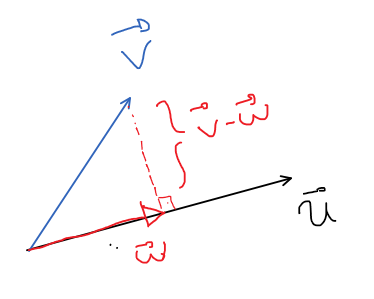
\includegraphics[width=0.4\linewidth]{Imagens/projOrtog}
		\caption{Projeção ortogonal de $v$ em $u$}
		\label{fig:projortog}
	\end{figure}
	
	Precisamos de duas premissas, as quais são facilmente observadas na figura acima:
	\begin{align*}
		&w=\alpha\cdot u\\
		&\langle u,v-w \rangle=0
	\end{align*}
	A maneira de encontrar, explicitamente, $w$ em função de $u$ e $v$, com base nessas premissas, está descrita abaixo:
	\begin{align*}
		\langle u,v-w \rangle&=0\\
		\langle u,v-\alpha u \rangle&=0\\
		u\cdot v - \alpha\cdot u\cdot u&=0\\
		\alpha\cdot u\cdot u&=u\cdot v\\
		\alpha&=\dfrac{u\cdot v}{u\cdot u}
	\end{align*}
	
	Sendo assim, temos:
	\begin{equation*}
		w=\left(\dfrac{u\cdot v}{u\cdot u}\right) \cdot u
	\end{equation*}
	
	Note que o resultado dos produtos internos entre parênteses é um número, garantindo que $w$ e $u$ são paralelos.
	
	\subsubsection{Matriz de Projeção sobre o vetor $u$}
	
	
	Podemos encapsular a projeção ortogonal sobre um vetor $u$ em uma matriz $P$, da seguinte forma:
	\begin{align*}
		w&=\left(\dfrac{u\cdot v}{u\cdot u}\right) \cdot u\\
		&=\left(\dfrac{u^{T} v}{u^{T} u}\right) \cdot u\\
		&=u\left(\dfrac{u^{T} v}{u^{T} u}\right)\\
		&=\left(\dfrac{u u^{T}}{u^{T} u}\right)v\\
		&=P\cdot v
	\end{align*}
	
	\subsubsection{Exemplo:}
	Calcule a matriz de projeção sobre o vetor $u=(1,-1,1)$
	\begin{align*}
		P&=\left(\dfrac{u u^{T}}{u^{T} u}\right)\\
		P&=\dfrac{1}{3}\begin{pmatrix}
			1 \\
			-1 \\
			1
		\end{pmatrix}\begin{pmatrix}
			1 & -1 & 1
		\end{pmatrix}\\
		P&=\dfrac{1}{3}\begin{pmatrix}
			1 & -1 & 1\\
			-1 & 1 & -1\\ 
			1 & -1 & 1
		\end{pmatrix}
	\end{align*}
	
	\subsubsection{Propriedades:}
	
	A matriz $P$ definida possui as seguintes propriedades:
	\begin{enumerate}
		\item $P$ é simétrica
		\item $P^2=P$
		\item Posto($P$)=1
	\end{enumerate}
	
	\subsection{Projeção Ortogonal sobre um subespaço qualquer}
	Considere as matriz $A$ e o vetor $b$ definidos abaixo. Além disso, seja $w$ a projeção ortogonal de $b$ sobre o espaço coluna de $A$.
	\begin{equation*}
		A=\begin{pmatrix}
			a_{11} & a_{12} \\
			a_{21} & a_{22}\\
			a_{31} & a_{32} 
		\end{pmatrix},b=\begin{pmatrix}
			b_{11} \\
			b_{21} \\
			b_{31}
		\end{pmatrix}	
	\end{equation*}
	
	\begin{figure}[H]
		\centering
		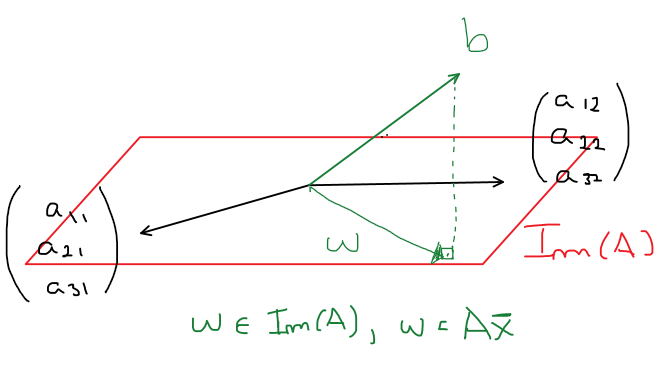
\includegraphics[width=0.4\linewidth]{Imagens/projOrtogEsp}
		\caption{projeção ortogonal sobre imagem de $A$}
		\label{fig:projortogesp}
	\end{figure}
	
	
	Note que:
	\begin{enumerate}
		\item o vetor $b-w$ é ortogonal ao espaço coluna de $A$
		\item o vetor $b-A\overline{x}$ é ortogonal ao espaço coluna de $A$, sendo $w=A\overline{x}$.
		\item Logo, $b-A\overline{x}\in $ Núcleo da Transposta de A
		\item $A^T(b-A\overline{x})=0$
		\item $A^Tb=A^TA\overline{x} \rightarrow$ Equação Normal
	\end{enumerate}
	\textbf{Obs:} se as colunas de $A$ são $LI$, então $A^TA$ é inversível.
	
	Com isso, chegamos na matriz de projeção sobre o espaço coluna de $A$:
	\begin{equation*}
		P=A\left(A^TA\right)^{-1}A^T
	\end{equation*}
	\subsection{Conclusão}
	Neste capítulo foram apresentados conceitos projeções ortogonais sobre u vetor e sobre um subespaço vetorial qualquer.
	
	\section{Mínimos Quadrados}
	
	\subsection{Motivação}
	
	Como já sabemos, estamos quase sempre interessados em resolver sistemas do tipo $Ax=b$. No entanto, há casos em que a solução deste sistema é impossível. Por exemplo, se o nosso sistema linear for um sistema linear de equações incompatíveis.
	
	\textbf{Def:} Sistemas lineares incompatíveis são sistemas de $m$ equações e $n$ incógnitas onde $m>n$. Outra maneira de olhar para essa definição é pensar em matrizes $A_{mxn}$, as quais possuem $m$ linhas (equações) e $n$ colunas (incógnitas). Sabemos que sistemas desse tipo não possuem solução.
	
	O que fazer, pode ser feito, além de abandonar o problema e ir dormir em paz, é procurar uma solução aproximada de tal modo que o \textbf{erro} desta solução seja o menor possível. 
	
	\textbf{Def:} o erro de uma solução aproximada de um sistema $Ax=b$, é definido como:
	\begin{equation*}
		||Ax-b|| \mbox{ , onde b é a solução real e Ax é a solução aproximada.}
	\end{equation*}
	
	Perceba que, para casos em que podemos encontrar a solução real do sistema, esse erro é zero, uma vez que $Ax=b$, logo $||Ax-b||=0$.
	
	Mas e quando não é possível encontrar a solução?
	
	\subsection{Relembrando Projeções Ortogonais}
	
	Lembre-se da capítulo passado sobre projeções ortogonais e acrescente um detalhe.
	
	\begin{figure}[H]
		\centering
		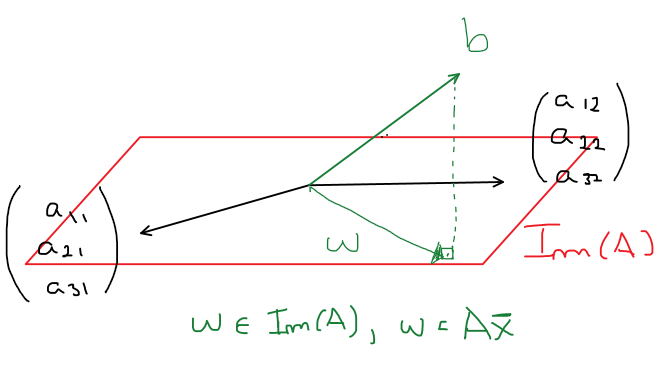
\includegraphics[width=0.4\linewidth]{Imagens/projOrtogEsp}
		\caption{projeção ortogonal sobre imagem de $A$}
		\label{fig:projortogesp}
	\end{figure}
	
	No âmbito de minimização de erro, podemos pensar que queremos a menor distância entre a solução real e a aproximada. Sendo assim, a \textit{Projeção Ortogonal} aprendida de mostra muito adequada para esse problema de aproximação.
	
	A própria equação normal $A^TA\overline{x}=A^Tb$ relaciona esses valores. Tenha isso em mente.
	
	\subsection{Mínimos Quadrados}
	
	Uma vez que o sistema linear $Ax=b$ é incompatível, sabemos que $b \notin Col(A)$. Sendo assim, já sabemos que a melhor solução, a que minimiza o erro, será a solução $\overline{x}$ tal que:
	\begin{equation*}
		A\overline{x}=Proj_{Col(A)}b
	\end{equation*}
	
	Como vimos na aula anterior, podemos definir uma matriz $P$ de projeção sobre o espaço coluna de $A$. Utilizando essa informação, chegamos no seguinte sistema:
	\begin{equation*}
		A\overline{x}=Pb
	\end{equation*}
	
	Este sistema, agora, é compatível e possui uma solução.
	
	Vejamos, por fim, um exemplo prático de como calcular a melhor reta para um dado conjunto de pontos (regressão linear).
	
	\subsubsection{Exemplo:}
	Encontre a reta que melhor interpola os seguintes pontos:
	\begin{table}[]
		\centering
		\begin{tabular}{|l|l|}
			\hline
			x  & y \\ \hline
			-1 & 1 \\ \hline
			1  & 1 \\ \hline
			2  & 3 \\ \hline
		\end{tabular}
	\end{table}
	
	Dados esses pontos, podemos montar o seguinte sistema linear $Ax=y$:
	\begin{equation*}
		\begin{pmatrix}
			1 & x_{1} \\
			1 & x_{2}\\
			1 & x_{3} 
		\end{pmatrix}\cdot 
		\begin{pmatrix}
			b \\
			a 
		\end{pmatrix}=
		\begin{pmatrix}
			y_1 \\
			y_2 \\
			y_3
		\end{pmatrix}
	\end{equation*}
	\begin{equation*}
		\begin{pmatrix}
			1 & -1 \\
			1 & 1\\
			1 & 2 
		\end{pmatrix}\cdot 
		\begin{pmatrix}
			b \\
			a 
		\end{pmatrix}=
		\begin{pmatrix}
			1 \\
			1 \\
			3
		\end{pmatrix}
	\end{equation*}
	
	Rescrevemos como da seguinte maneira:
	\begin{align*}
		Ax&=y\\
		A^TAx&=A^Ty
	\end{align*}
	
	Colocando valores:
	\begin{equation*}
		\begin{pmatrix}
			1 &1 &1\\
			-1 &1& 2
		\end{pmatrix}
		\begin{pmatrix}
			1 & -1 \\
			1 & 1\\
			1 & 2 
		\end{pmatrix}\cdot 
		\begin{pmatrix}
			b \\
			a 
		\end{pmatrix}=
		\begin{pmatrix}
			1 &1 &1\\
			-1 &1& 2
		\end{pmatrix}
		\begin{pmatrix}
			1 \\
			1 \\
			3
		\end{pmatrix}
	\end{equation*}
	
	Resolvendo o sistema, encontramos $a=\dfrac{4}{7}$ e $b=\dfrac{9}{7}$.\\
	
	Logo, a reta desejada é: $r(x)=\dfrac{4}{7}\cdot x + \dfrac{9}{7}$
	
	\subsection{Conclusão}
	Neste capítulo foi relembrado o conceito de projeções ortogonais sobre um subespaço vetorial qualquer e apresentado o algoritmo de Mínimos Quadrados.
	
	
	\section{Matrizes Ortogonais, Ortogonalização de Grand-Schimdt e Fatoração QR}
	
	\subsection{Matrizes Ortogonais}
	
	Para definir uma matriz ortogonal, precisamos lembrar o que é um conjunto de vetores, ou uma base, se quisermos, ortonormal.\\
	
	\textbf{Def:} uma base $\beta$ de vetores de $R^n$ é dita ortonormal se todos os vetores que a formam possuem, simultaneamente, norma 1 e são ortogonais entre si.\\
	
	Com essa definição, podemos definir tranquilamente uma Matriz Ortogonal.\\
	
	\textbf{Def:} Uma Matriz Ortogonal $A$ é uma matriz cujas colunas formam uma base ortonormal. \\
	
	Algumas propriedades das matrizes ortogonais são importantes para nosso curso.
	
	\subsubsection{Propriedades}
	
	\textbf{(1)} Toda matriz ortogonal $Q$ satisfaz $Q^{T}Q=I$. Dessa propriedade, nota-se que $Q^T=Q^{-1}$\\
	
	\textit{Prova:} note que uma multiplicação matricial é, de certo modo, um produto interno entre as colunas e linhas das matrizes. Sendo assim, como as colunas de $Q$ são ortonormais, $\langle v_i,v^{T}_{j} \rangle=0 \forall i\neq j$, sendo $v_i$ os vetores da coluna de $Q$ e $v_j$ os vetores linhas de $Q^T$. A partir disso mostramos que $Q^TQ=I$.  \\
	
	\textbf{(2)} A multiplicação de uma matriz ortogonal por um vetor preserva o comprimento do vetor $\rightarrow ||Qx||=||x||$. \\
	
	\textit{Dem:} $||Qx||^2 = \langle Qx,Qx \rangle=(Qx)^TQx=x^TQ^TQx=x^Tx=||x||^2$\\
	
	\textbf{(3))} O ângulo entre vetores se preserva por matriz ortogonal.\\
	
	\textit{Dem:} $cos\theta=\dfrac{\langle Qu,Qv \rangle}{||Qu|||Qv|||}=\dfrac{uQ^TQv}{||u|||v|||}=\dfrac{u^Tv}{||u|||v|||}$
	
	\subsection{Ortogonalização de Grand Schimdt}
	
	O processo de ortogonalização de Grand-Schimdt consiste em uma estratégia para, a partir de uma base qualquer $\{a_1,...,a_n\}$, obter uma base ortonormal $\{q_1,...q^n\}$ para o espaço gerado pela base $a$. Temos a seguinte construção:
	\begin{align*}
		&a_1^{'}=a_1 \rightarrow q_1=\dfrac{a_1^{'}}{||a_1^{'}||}\\
		&a_2^{'}=a2-(q_1^Ta_2)q_1 \rightarrow q_2=\dfrac{a_2^{'}}{||a_2^{'}||}\\
		&a_3^{'}=a3-(q_1^Ta_3)q_1 -(q_2^Ta_3)q_2\rightarrow q_3=\dfrac{a_3^{'}}{||a_3^{'}||}\\
		&a_n^{'}=an-(q_1^Ta_n)q_1 -...-(q_{n-1}^Ta_n)q_{n-1}\rightarrow q_n=\dfrac{a_n^{'}}{||a_n^{'}||}
	\end{align*}
	
	
	\subsection{Fatoração QR}
	
	O processo de ortogonalização de Grand Schimdt nos entrega uma fatoração conhecida como \textbf{fatoração $A=QR$}. Não é difícil imaginar que a matriz $Q$ desta fatoração será a matriz cujas colunas são a base $\{q_1,...q^n\}$ obtida no processo de ortogonalização e $A$ é a matriz cujas colunas são a base $\{a_1,...,a_n\}$.\\
	
	Antes de definirmos a matriz $R$, lembremos:\\	
	
	Se $\{q_1,...q^n\}$ é base ortonormal de $R^N$ e $b$ pertence a esse espaço gerado, então...
	\begin{equation*}
		b=c_1q_1+c_2+q_2+...+c_nq_n
	\end{equation*}
	onde
	\begin{equation*}
		c_1=q_1^Tb, c_2=q_2^Tb... c_n=q_n^Tb
	\end{equation*} 
	
	Vejamos como construir a matriz $R$ para o caso de uma base do $R^3$. Esse procedimento é facilmente generalizado para $R^N$.
	
	\textbf{Exemplo:} Seja $\{a,b,c\}$ base para o $R^3$ e $\{q_1,q_2,q^3\}$ base ortonormal obtida via ortogonalização de Grand Schimdt a partir da base $\{a,b,c\}$.\\
	
	Temos que:\\
	
	$a=(q_1^Ta)q_1+(q_2^Ta)q_2+(q_3^Ta)q_3=(q_1^Ta)q_1$\\
	
	A primeira coluna de $R$ será, então, $(q_1^{T}a,0,0)^T$\\
	
	$b=(q_1^Tb)q_1+(q_2^Tb)q_2+(q_3^Tb)q_3=(q_1^Tb)q_1+(q_2^Tb)q_2$\\
	
	A segunda coluna de $R$ será, então, $(q_1^{T}a,q_2^Tb,0)^T$\\
	
	$a=(q_1^Tc)q_1+(q_2^Tc)q_2+(q_3^Tc)q_3$\\
	
	A terceira coluna de $R$ será, então, $(q_1^{T}a,q_2^Tb,q_3^Tc)^T$\\
	
	Logo, $R=\begin{pmatrix}
		q_1^{T}a & q_1^{T}a & q_1^{T}a\\
		0 &  q_2^Tb& ,q_2^Tb\\ 
		0 & 0 & q_3^Tc
	\end{pmatrix}$
	
	\subsection{Conclusão}
	Neste capítulo apresentados os conceitos de Matriz Ortogonal, Processo de Ortogonalização de Grand-Schimdt e Fatoração $A=QR$.
	
	
	\section{Polinômio Característico e Teorema de Cayley Hamilton}
	
	\subsection{Polinômio Característico}
	
	O polinômio característico de uma matriz é um conceito de extrema importância para a Álgebra Linear. É a partir dele que poderemos definir os conceitos de autovalores e autovetores, que, por sua vez, também são muito importantes. Esses conceitos surgem nas mais variadas aplicações, desde diagonalização de matriz e transformações lineares até cálculo funcional e sistemas de equações de diferenças.
	
	Dito isso, passeamos para a definição de polinômio característico.\\
	
	\textbf{Def:} seja $A$ uma matriz quadrada de dimensões $nxn$. O polinômio característico dessa matriz é definido como:
	\begin{equation*}
		p(\lambda)=det(\lambda I-A)\mbox{ , onde I é a matriz Identidade de }R^n, \lambda \in R
	\end{equation*}\\
	
	\textbf{Ex:} Calcule o polinômio característico da matriz $A$ abaixo:
	\begin{equation*}
		A=\begin{pmatrix}
			a&b\\
			c&d
		\end{pmatrix}
	\end{equation*}
	\begin{align*}
		det(\lambda I-A)&=det
		\begin{pmatrix}
			\lambda-a&b\\
			c&\lambda-d
		\end{pmatrix}=\\
		&= (\lambda-a)(\lambda-d)-cb\\
		&= \lambda^2 -(a+d)\lambda+(ad-bc)
	\end{align*}
	
	Podemos fazer alguns comentários interessantes sobre esse resultado:
	\begin{enumerate}
		\item O último termo entre parênteses é o determinante da matriz $A$ original.
		\item $p(0)=det(0\cdot I-A)=det(-A)=det(A\cdot(-I))=det(A)\cdot det(-I)=det(A)\cdot(-1)^n$
	\end{enumerate}
	
	\subsection{Teorema de Cayley Hamilton}
	
	O teorema de Cayley Hamilton é simples de ser demonstrado e diz o seguinte:\\
	
	\textbf{Def:} Se $A$ é uma matriz quadrada $nxn$ e $p(\lambda)$ seu polinômio característico, então $p(A)=0$.\\
	
	\textit{Demonstração:}
	\begin{align*}
		p(\lambda)&=det(\lambda I-A)\\
		p(A)&=det(A\cdot I-A)=det(0)=0
	\end{align*}
	
	Esse teorema possui algumas aplicações interessantes que justificam seu estudo. Vejamos duas delas.
	\subsubsection{Aplicação 1 - Cálculo da Inversa}
	
	Vamos direto para um exemplo. Seja a matriz $A$ abaixo. Calcule sua inversa via Teorema de Cayley Hamilton.
	\begin{equation*}
		A=\begin{pmatrix}
			1&-1\\
			2&4
		\end{pmatrix}
	\end{equation*}
	
	Temos que o polinômio característico dessa matriz é $p(\lambda)=\lambda^2-5\lambda+6$.
	
	A partir de $p(\lambda)$ podemos verificar facilmente que a matriz $A$ é inversível uma vez que o termo independente do polinômio, que corresponde ao determinante de $A$ é diferente de 0. Aplicando o Teorema de Cayley Hamilton temos a seguinte equação. Note que precisamos multiplicar o termo independente pela matriz identidade para a equação fazer sentido!
	
	\begin{equation*}
		p(A)=0\rightarrow A^2-5A+6I=0
	\end{equation*}
	
	Desenvolvendo...
	
	\begin{align*}
		A^2-5A&=-6I\\
		A^{-1}(A^2-5A)&=-6A^{-1}I\\
		A-5I&=-6A^{-1}\\
		A^{-1}&=-\dfrac{1}{6}(A-5I)
	\end{align*}
	
	Calculando a inversa do enunciado temos a seguinte resposta:
	\begin{equation*}
		A^{-1}=\dfrac{1}{6}
		\begin{pmatrix}
			4&1\\
			-2&1
		\end{pmatrix}
	\end{equation*}
	
	Sabendo que a demonstração genérica do cálculo da matriz inversa via Teorema de Cayley Hamilton não é difícil, ela ficará como um desafio para quem quiser! Qualquer dúvida, não hesite em entrar em contato comigo.
	
	\subsubsection{Aplicação 2 - Divisão de Polinômios}
	
	Vejamos como o conhecimento desse Teorema, somado À divisão de polinômios, nos tora capazes de simplificar a aplicação de um polinômio qualquer em $A$.
	
	Considere $p_2(\lambda)=\lambda^r+a_{r-1}\lambda^{r-1}+...+a_0$ um polinômio qualquer. Podemos simplificar o cálculo de $p_2(A)$ da seguinte forma:
	\begin{equation*}
		p_2(A)=p(A)\cdot q+ s
	\end{equation*}
	
	A equação acima é a expressão de uma divisão de polinômios, sendo $p(A)$ o polinômio característico de $A$ aplicado em $A$, o que resulta em 0, obviamente, $q$ é o quociente e $s$ é o resto da divisão. Lembremo-nos que o grau de $p_2(A)$ é $r$, de $p(A)$ é $n$, de $q$ é $r-n$ e de $s$ é menor que $n$.
	
	A partir da aplicação do Teorema de Cayley Hamilton, teremos:
	\begin{equation*}
		p_2(A)=p(A)\cdot q+ s=0q+s=s
	\end{equation*}
	
	
	Vamos a um exemplo!
	
	Seja $A$ a matriz abaixo, $p(\lambda)$ seu polinômio característico e $p_2(\lambda)$ um polinômio definido abaixo. Calculemos $p_2(A)$.
	\begin{align*}
		A&=\begin{pmatrix}
			1&-1\\
			2&4
		\end{pmatrix}\\
		p(\lambda)&=\lambda^2-5\lambda+6\\
		p_2{\lambda}&=\lambda^7-5\lambda^6+6\lambda^5-2\lambda^3+11\lambda^2-16\lambda+5
	\end{align*}
	
	A imagem abaixo exibe o cálculo de $p_2(\lambda)$ simplificado. Peço perdão pela letra...
	
	\begin{figure}[H]
		\centering
		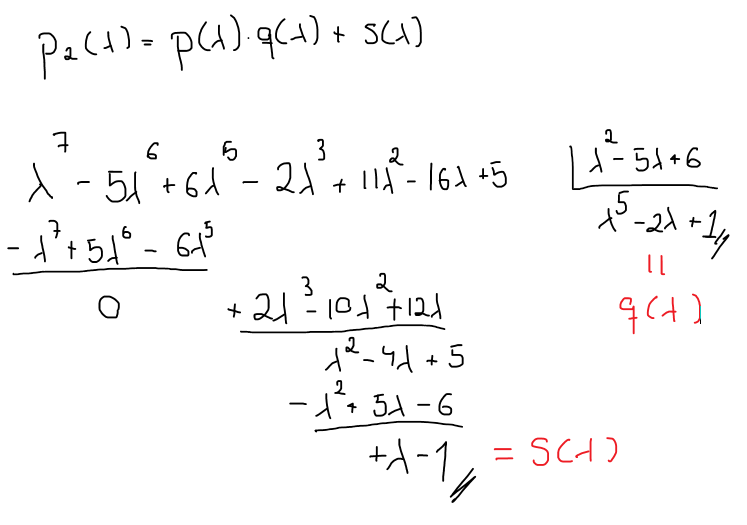
\includegraphics[width=1\linewidth]{Imagens/aplicacao2}
		\caption{Cálculo de $q(\lambda)$ e $s(\lambda)$}
		\label{fig:aplicacao2}
	\end{figure}
	
	Com isso, temos que $p_2(\lambda)=\lambda-1$.\\
	
	Logo,  $p_2(A)=A-1I=\begin{pmatrix}
		0 & -1 \\
		2 & 3
	\end{pmatrix}
	$
	
	\subsection{Conclusão}
	Neste capítulo apresentados os conceitos de  Polinômio Característico e Teorema de Cayley Hamilton, além de estudadas algumas aplicações importantes desse teorema. Em seguida, veremos as definições de autovalores e autovetores, uma aula que eu costumo chamar, informalmente, de "autotudo".
	
	\section{Auto-Tudo}
	
	\subsection{Autovalores e Autovetores}
	
	Como esses conceitos são apresentados e bem trabalhados em Álgebra Linear 1, podemos partir direto para a definição.\\
	
	\textbf{Def:} seja $A$ uma transformação linear de $R^n$ para $R_n$. Chamamos de autovalor o número real $\lambda$ que satisfaz:
	\begin{equation*}
		T(v)=\lambda v
	\end{equation*}
	
	Além disso, chamamos $v$ de autovetor associado ao autovalor $\lambda$.\\
	
	A partir dessas definições, podemos, em seguida, definir o conceito de subespaço característico.\\
	
	\textbf{Def:} o conjunto de todos os autovetores de $A$ associados a um autovalor $\lambda$ é denominado subespaço característico de $A$ associado a $\lambda$, também representado por $A_{\lambda}$.\\
	
	Dado o nome deste subespaço vetorial, podemos supor que o polinômio característico da matriz $A$ possui alguma relação com seus autovalores e autovetores. Essa relação se dá pelo fato de que as raízes do polinômio característico de $A$, $p(\lambda)=0$ são, justamente, os autovalores de $A$. Note que, devido a essa maneira de calcular os autovalores, sabemos que uma matriz $A$ de dimensões $n\times n$ terá sempre, no máximo, $n$ autovalores. Com os autovalores em mãos, a maneira mais trivial de calcular os autovetores associados é por meio da própria definição de autovetor.
	
	Além disso, os autovetores $v_i$ estão associados aos autovalores $\lambda_i$ da seguinte forma:
	\begin{equation*}
		(\lambda_iI-A)v_i=0
	\end{equation*}
	
	o que é o mesmo que dizer que...
	\begin{equation*}
		v_i \in Nucleo(\lambda_iI-A)
	\end{equation*}
	
	Apresentemos mais algumas definições importantes conhecidas como multiplicidades.\\
	
	\textbf{Def:} Multiplicidade Algébrica de $\lambda$ corresponde à quantidade de raízes de $p(\lambda)$ que são iguais a $\lambda$.
	
	\textbf{Def:} Multiplicidade Geométrica de $\lambda$ corresponde à dimensão do autoespaço $A_{\lambda}$.\\
	
	\textit{Exemplos:} vejamos os autovalores, autovetores e multiplicidades das matrizes a seguir.
	
	\begin{equation*}
		A=\begin{pmatrix}
			10 & -9 \\
			4 & -2
		\end{pmatrix}	
	\end{equation*}
	
	Calculando as raízes de seu polinômio característico encontramos $\lambda_1=\lambda_2=4$. Aplicando a definição, achamos o autovetor associado a esse autovalor $v_1=[1,2]^T$. 
	
	Logo, a multiplicidade algébrica do autovalor 2 é 2, uma vez que sã duas raízes iguais a 2 e a multiplicidade geométrica é igual a 1, pois há apenas 1 autovetor.\\
	
	\begin{equation*}
		A=\begin{pmatrix}
			1 & 0 \\
			0 & 1
		\end{pmatrix}	
	\end{equation*}
	
	Calculando as raízes de seu polinômio característico encontramos $\lambda_1=\lambda_2=1$. Aplicando a definição, achamos os autovetores associados a esses autovalores $v_1=[1,0]^T$ e $v_2=[0,1]^T$. 
	
	Logo, a multiplicidade algébrica do autovalor 1 é 2, uma vez que sã duas raízes iguais a 2 e a multiplicidade geométrica é igual a 2, pois há 2 autovetores LI.
	
	\subsection{Diagonalização}
	
	Novamente, vamos direto para a definição.\\
	
	\textbf{Def:} uma matriz $A_{n\times n}$ é dita diagonalizável se existe uma matriz $P$ tal que $P^{-1}AP=D$, onde $D$ é uma matriz diagonal.
	
	Se $A$ possui apenas autovetores LI, então:
	\begin{equation*}
		P=\begin{pmatrix}
			| & | & |\\
			v_1 & v_2 & v_n\\
			| & | & |
		\end{pmatrix} \mbox{ e }
		D=\begin{pmatrix}
			\lambda_1 & 0 & 0 \\
			0 & \lambda_2 & 0 \\
			0 & 0 & \lambda_n
		\end{pmatrix}
	\end{equation*}
	
	O procedimento para encontrar a diagonalização de uma matriz $A$ é:
	\begin{enumerate}
		\item Encontrar os autovetores LI de $A$, se houver
		\item Construir a matriz $P$ com esses autovetores nas colunas
		\item Construir a matriz $D$ como $P^{-1}AP$.
	\end{enumerate}
	
	Vamos enumerar, e não demonstrar, alguns teoremas importantes. 
	
	\textbf{Teorema:} Se $A_{n\times n}$ é quadrada, então são equivalentes as seguintes proposições:
	\begin{enumerate}
		\item $A$ é diagonalizável
		\item $A$ possui $n$ autovalores LI, ou seja, $A=MG$
		\item $R^n=A_{\lambda1}+A_{\lambda2}+...+A_{\lambda n}$ 
	\end{enumerate}
	
	\textbf{Teorema:} se todos os autovalores de $A$ são distintos, então $A$ é diagonalizável.
	
	\textbf{Teorema:} Os autovetores associados a autovalores distintos são LI.
	
	\subsection{Potência de Matrizes}
	
	O conhecimento do conceito de autovalor é um enorme facilitador para o cálculo de potência de matrizes. Vejamos o motivo.
	
	Partindo da definição de uma matriz diagonal, vamos mostrar como calcular $A^2$.
	
	\begin{align*}
		A&=PDP^{-1}\\
		A^2&=(PDP^{-1})^2\\
		A^2&=PDP^{-1}PDP^{-1}\\
		A^2&=PDDP^{-1}\\
		A^2&=PD^2P^{-1}
	\end{align*}
	
	Podemos, facilmente, generalizar: $A^n=PD^nP^{-1}$.
	
	Outra pergunta interessante é: quais os autovalores de $A^n$?
	
	A demonstração é muito simples e similar à intuição dada pela potência de matriz acima, então me abstenho que realizá-la aqui. Sendo assim, respondemos que os autovalores de $A^n$ são iguais a $\lambda^n$, sendo $\lambda$ os autovalores de $A$. 
	
	\subsection{Conclusão}
	Neste capítulo foram apresentados os conceitos de  Autovalores e Autovetores, além de algumas aplicações desses conceitos, como a Diagonalização de Matrizes. Nas próximas aulas todos esses conceitos serão muito utilizados para estudarmos cálculo funcional. 
	
	\section{Cálculo Funcional: Caso Diagonalizável}
	
	\subsection{Algumas Definições}
	
	Considere uma matriz quadrada $A_{n\times n}$. O cálculo funcional associa, a cada função, uma matriz $f(A)$. Por exemplo, seja $f: R\rightarrow R$ a função exponencial $f(x)=e^x$. Se $A$ for nossa matriz, quanto vale $f(A)=e^A$?
	
	Como não é ementa deste curso, vamos apenas definir uma série de potências e a Série de Taylor, bem como fornecer as séries de Taylor para algumas funções usuais. Para mais informações em relação a essas séries, a disciplina de Cálculo 4 é a ideal.
	
	\textbf{Def:} Série de Potências é definida por
	\begin{equation*}
		f(x)=\sum_{n=0}^{\inf}a_{n}x^n
	\end{equation*}
	
	\textbf{Def:} Série de Taylor de uma função $f(x)$ é definida como
	\begin{equation*}
		f(x)=\sum_{n=0}^{\inf}\dfrac{f^n(x_0)}{n!}(x-x_0)n
	\end{equation*}
	
	onde $f^n(x)$ é a n-ésima derivada de $f(x)$ em relação a $x$.
	
	Temos, por exemplo, que a série de Taylor para as funções exponencial, seno e cosseno é:
	\begin{align*}
		e^x=\sum_{n=0}^{\inf}\dfrac{1}{n!}x^n&=1+x+\dfrac{1}{2!}x^2+\dfrac{1}{3!}x^3+...\\
		sen(x)&=\sum_{n=0}^{\inf}\dfrac{(-1)^n}{(2n+1)!}x^{2n+1}\\
		cos(x)&=\sum_{n=0}^{\inf}\dfrac{(-1)^n}{(2n)!}x^{2n}
	\end{align*}
	
	Uma vez definidas essas séries para algumas funções, podemos nos perguntar, novamente, como calcular a exponencial de $A$. No entanto, podemos responder essa pergunta de uma forma um pouco mais adequada.
	\begin{equation*}
		e^A=I+A+\dfrac{1}{2!}A^2+\dfrac{1}{3!}A^3+...+\dfrac{1}{n!}A^n+...
	\end{equation*}
	
	A partir dessa expressão, podemos calcular "facilmente" a exponencial de uma matriz! Para, de fato, facilitar nossos cálculos, vejamos o caso em que $A$ é uma matriz diagonalizável.
	
	\subsection{Caso Diagonalizável}
	
	Seja $A_{n\times n}$ uma matriz quadrada diagonalizável. Ou seja, temos $A=SDS^{-1}$. Adicionando essa informação à série de Taylor da exponencial, teremos o seguinte:
	
	\begin{align*}
		e^A&=I+A+\dfrac{1}{2!}A^2+\dfrac{1}{3!}A^3+...+\dfrac{1}{n!}A^n+...\\
		e^A&=I+SDS^{-1}+\dfrac{1}{2!}SDS^{-1}SDS^{-1}+\dfrac{1}{3!}SDS^{-1}SDS^{-1}SDS^{-1}+...+\dfrac{1}{n!}(SDS^{-1})^n+...\\
		e^A&=SIS^{-1}+SDS^{-1}+\dfrac{1}{2!}SD^2S^{-1}+\dfrac{1}{3!}SD^3S^{-1}+...+\dfrac{1}{n!}SD^nS^{-1}+...\\
		e^A&=S(I+D+\dfrac{1}{2!}D^2+\dfrac{1}{3!}D^3+...)\\
		e^A&=Se^DS{-1}
	\end{align*}
	
	Sabemos calcular $e^D$, basta aplicar a função exponencial nas entradas da diagonal principal, fazendo $e^{\lambda_i}$. Além disso, também sabemos calcular a matriz $S$, basta pssuirmos os autovetores de $A$.
	
	De forma geral, se $f$ está definida para os autovalores de $A$ e $A$ é diagonalizável, então:
	\begin{equation*}
		f(A)=Sf(D)S^{-1}
	\end{equation*}
	
	Para finalizar, enumeremos algumas observações importantes:
	\begin{itemize}
		\item Se $\lambda$ é autovalor de $A$, então $e^\lambda$ é autovalor de $e^A$
		\item $det(e^A)=e^\lambda_1e^\lambda_2...e^\lambda_n=e^(\lambda_1+\lambda_2+...+\lambda_n)=e^{tr(A)}$
		\item $e^A$ é sempre inversível, pois $det(e^A)\neq 0$
	\end{itemize}
	
	\subsection{Conclusão}
	Neste capítulo foram apresentados os conceitos de cálculo funcional e a explicação de seu caso diagonaizável. Note que ganhamos um ferramental poderoso, pois podemos aplicar (quase) qualquer função a uma matriz. Nas próximas aulas continuaremos explorando o cálculo funcional. 
	
	\section{Cálculo Funcional: Caso Não Diagonalizável}
	
	\subsection{Lembrando a aula anterior}
	
	Na última semana foi discutido o cálculo funcional em seu caso diagonalizável. Lembremos:
	
	Dada $f$ uma função definida nos autovalores de $A_{n\times n}$	e $f(x)=\sum_{i=0}^{\inf}a_ix^i$, então, $f(A)=a_0I+a_1A+a_2A^2+...$\\
	
	Se $A=SDS^{-1}$, então $f(A)=Sf(D)S^{-1}$.
	
	\subsection{Caso não diagonalizável}
	
	Para calcular $f(A)$, sendo $A_{n\times n}$ uma matriz não diagonalizável, seguiremos o seguinte algoritmo:
	\begin{enumerate}
		\item Determinar $p(\lambda)=(\lambda I-A)$
		\item Determinar os autovalores de $A$ com suas respectivas multiplicidades
		\item Determinar o polinômio $q$ de grau $n-1$, tal que, para cada autovalor $\lambda_i$:
		\begin{align*}
			q(\lambda_i)&=f(\lambda_i)\\
			q'(\lambda_i)&=f'(\lambda_i)\\
			q^{m_i-1}(\lambda_i)&=f^{m_i-1}(\lambda_i)
		\end{align*}, onde $m_i$ é a multiplicidade de $\lambda_i$
		\item $f(A)=q(A)$
	\end{enumerate}
	
	\subsubsection{Exemplo 1}
	
	Seja $A$ a matriz abaixo. Calcule $f(A)$ sabendo que $f(x)=x^{150}$.
	\begin{equation*}
		A=\begin{pmatrix}
			3 & 1 \\
			0 & 3
		\end{pmatrix}
	\end{equation*}
	
	\textbf{Solução:}
	
	É fácil calcular que os autovalores de $A$ são $\lambda_1=3$ com multiplicidade $m_1=2$.
	
	Neste caso, temos $n=2$, logo o polinômio $q$ terá grau $n-1=2-1=1$: $q(x)=ax+b$. Precisamos calcular $a$ e $b$.
	
	Sabemos que 
	\begin{equation*}
		\begin{cases}
			q(3)=f(3)\\q'(3)=f'(3)
		\end{cases}
	\end{equation*}
	
	Com isso, temos:
	
	\begin{equation*}
		\begin{cases}
			3a+b=3^{150}\\a=150\cdot 3^{149}
		\end{cases}
	\end{equation*}
	
	Bastam algumas contas para calcular $a$ e $b$ e teremos nosso polinômio:
	\begin{equation*}
		q(x)=150\cdot 3^{149}\cdot x-149\cdot 3^{150}
	\end{equation*}
	
	Por fim, fazemos $f(A)=q(A)$:
	\begin{align*}
		A^{150}&=150\cdot 3^{149}\cdot A-149\cdot 3^{150}\cdot I\\
		A^{150}&=\begin{pmatrix}
			1\cdot 3^{150}&150\cdot 3^{149}  \\
			0& 3^{150}
		\end{pmatrix}	
	\end{align*}
	
	\subsection{Justificativa Intuitiva}
	
	Vejamos uma justificativa pouco formal, para o fato de $f(A)=q(A)$.
	
	Se $f$ for um polinômio, temos que:
	\begin{align*}
		h(x)&=f(x)-q(x)\\
		h(\lambda_i)=h'(\lambda_i)&=...=h^{m_i-1}(\lambda_i)=0 \mbox{ pois } h(\lambda_i)=f(\lambda_i)-q(\lambda_i)
	\end{align*}
	
	Note que todos os autovalores são raízes de $h(x)$, logo,
	\begin{align*}
		h(x)&=p(x)\cdot k(x)\\
		h(A)&=p(A)\cdot k(A)=0 \mbox{ lembre-se que p(A)=0}\\
		f(A)&-q(A)=0\\
		f(A)&=q(A)
	\end{align*}
	
	Se $f$ não for um polinômio, sabemos que ela pode ser aproximada por um, via Série de Taylor, por exemplo. Com isso, podemos descrever uma justificativa similar para verificar que a propriedade $f(A)=q(A)$ vale.
	
	\subsection{Conclusão}
	Neste capítulo foi o cálculo funcional para o caso diagonalisável e apresentado o caso não diagonalizável. Nas próximas aulas entraremos em sistemas de equações de diferenças.
	
	
	\section{Sistema de Equações de Diferenças}
	
	\subsection{Equações de Diferenças}
	
	Um sistema de equações de diferenças está associado à problemas do mundo discreto, onde temos informações pontuais de um sistema qualquer, em vez de informações contínuas. O exemplo que será abordado é o crescimento populacional.
	
	Considere a equação:
	\begin{equation*}
		y_{k+1}=f(y,k)\mbox{ onde }k\in N
	\end{equation*}
	
	A equação acima é uma equação de diferenças de \textbf{primeira ordem}, pois o valor $y_{k+1}$ depende apenas de $y_k$. Logo, uma equação de ordem $n$ é definida pelo fato de $y_{k+1}$ depender de $n$ valores anteriores.
	
	\textbf{Ex:} a equação $y_{k+1}=c\cdot y_k\mbox{ ,onde }k\in N \mbox{ e }c\in R$ possui solução da forma da sequência $y_1,y_2,y_3,...$
	
	Estamos interessados em buscar a solução geral da equação e avaliar seu comportamento quando $k\to \infty$.
	
	Para este exemplo, temos:
	\begin{align*}
		y_1&=c\cdot y_0\\
		y_2&=c\cdot y_1=c^2\cdot y_0\\
		y_k&=c\cdot y_{k-1}=c^k\cdot y_0
	\end{align*}
	
	Logo, avaliando no limite:
	\begin{equation*}
		\lim_{k\to \infty}y_k=\begin{cases}0\mbox{, se }|c|<1\\ y_0\mbox{, se }c=1\\ \not\exists\mbox{, se caso contrário} 
		\end{cases}
	\end{equation*}
	
	\subsection{Sistema de Equação de Diferenças}
	Podemos generalizar a definição de uma equação de diferenças, passando a enxergar $y_k$ não mais como um valor único, mas um vetor coluna de valores $u_k$:
	\begin{equation*}
		u_{k+1}=A\cdot u_k
	\end{equation*}
	onde $A$ é uma matriz $n\times n$ e $u_k\in R^n$.\\
	
	Dito isso, já sabemos que a solução geral é:
	\begin{equation*}
		u_{k+1}=A^k\cdot u_0
	\end{equation*}
	
	\subsubsection{Exemplos}
	Considere que, a cada ano, 10\% da população do Estado do Rio se ,uda para a capital e 20\% da população da capital se muda para outra cidade do estado.
	
	\textbf{(a)} Determine o sistema que modela a situação\\
	
	Podemos construir o seguinte vetor coluna $u_k=(y_k,z_k)^T$ onde $y_k$ é a população do estado e $z^k$ é a população da capital e $k$ é o ano. Com as informações do enunciado, podemos construir o seguinte sistema:
	\begin{equation*}
		\begin{cases}
			y+{k+1}=0.9\cdot y_k+0.2\cdot z_k\\
			z{k+1}=0.1\cdot y_k+0.8\cdot z_k
		\end{cases}
	\end{equation*}
	
	Pense e veja se você concorda com essas equações antes de continuar! Montar corretamente o sistema é essencial!
	
	Podemos, então, reescrever o sistema como:
	$u_{k+1}\begin{pmatrix}
		0.9 & 0.2 \\
		0.1 & 0.8
	\end{pmatrix}u_k$
	
	\textbf{(b)} A população em 2019 era de $y=15$ e $z=7$ milhões. Qual será a população nos próximos anos?\\
	
	\begin{align*}
		u_1&=\begin{pmatrix}
			0.9 & 0.2 \\
			0.1 & 0.8
		\end{pmatrix}\begin{pmatrix}
			15 \\
			7
		\end{pmatrix}=
		\begin{pmatrix}
			14.9 \\
			7.1
		\end{pmatrix}\\
		u_2&=\begin{pmatrix}
			0.9 & 0.2 \\
			0.1 & 0.8
		\end{pmatrix}\begin{pmatrix}
			14.9 \\
			7.1
		\end{pmatrix}=
		\begin{pmatrix}
			14.83 \\
			7.17
		\end{pmatrix}
	\end{align*}
	
	\textbf{(c)} Estude o comportamento do sistema quando $t\to \infty$.\\
	
	A estratégia para essa análise está expressa nos passos a seguir:
	
	\begin{align*}
		u_{k+1}&=A^ku_0\\
		u_{k+1}&=SD^{K}S^{-1}u_0\\
		u{k+1}&=S\begin{pmatrix}
			\lambda_1^k & 0 \\
			0 & \lambda_2^k
		\end{pmatrix}S^{-1}u_0
	\end{align*}
	
	O polinômio característico de $A$ é $p(\lambda)=\lambda^2-1.7\lambda+0.7$. Com ele, calculamos $\lambda_1=1$, $\lambda_2=0.7$, $v_1=\begin{pmatrix}
		2/3 \\
		1/3
	\end{pmatrix}$ e $v_2=\begin{pmatrix}
		1/3 \\
		-1/3
	\end{pmatrix}$.
	
	Com esses valores em mãos:
	
	\begin{equation*}
		A^k=\begin{pmatrix}
			2/3 & 1/3 \\
			1/3 & -1/3
		\end{pmatrix}
		\begin{pmatrix}
			1^k & 0 \\
			0 & 0.7^k
		\end{pmatrix}
		\begin{pmatrix}
			1 & 1 \\
			1 & -2
		\end{pmatrix}	
	\end{equation*}
	
	Portanto,
	\begin{align*}
		U_{k+1}&=\begin{pmatrix}
			2/3 & 1/3 \\
			1/3 & -1/3
		\end{pmatrix}
		\begin{pmatrix}
			1^k & 0 \\
			0 & 0.7^k
		\end{pmatrix}
		\begin{pmatrix}
			1 & 1 \\
			1 & -2
		\end{pmatrix}
		\begin{pmatrix}
			y_0 \\
			z_0
		\end{pmatrix}=...\\
		u_{k+1}&=(y_0+z+0)\begin{pmatrix}
			2/3 \\
			1/3
		\end{pmatrix}+0.7^k(y_0-2z_0)\begin{pmatrix}
			1/3 \\
			-1/3
		\end{pmatrix}
	\end{align*}
	
	Finalmente, avaliando o limite, temos:
	\begin{equation*}
		\lim_{k\to\infty}u_{k}=(y_0+z_0)\begin{pmatrix}
			2/3 \\
			1/3
		\end{pmatrix}
	\end{equation*}
	
	\subsubsection{Comentários Importantes}
	
	Podemos enumerar algumas considerações importantes sobre um sistema de equações de diferenças, principalmente em relação a sua estabilidade.\\
	
	Note que $u_k=c_1\lambda_1^kv_1+c_2\lambda_2^kv_2$.
	
	O sistema $u+{+1}=A^ku_k$ é:
	\begin{enumerate}
		\item Assintoticamente estável se $|\lambda_i|<1$, $\forall i$.
		\item Estável se $\exists j$, tal que $|\lambda_j|=1$ e $|\lambda_j|<1$ para os demais $j$.
		\item Instável se $|\lambda_1|>1$ para algum $i$.
	\end{enumerate}
	
	\subsection{Crescimento Populacional}
	
	Imagine que uma população de coelhos que possuem idade máxima de 15 anos. Dividimos a população em 3 faixas etárias: $[0,5],[5,10],[10,15]$. Sabemos que:
	\begin{itemize}
		\item 50\% de $[0,5]$ sobrevive
		\item 25\% de $[5,10]$ sobrevive
		\item De $[0,5]$ não há reprodução.
		\item De $[5,10]$ nascem 4 filhotes por fêmea.
		\item De $[10,15]$ nascem 3 filhotes por fêmea.
	\end{itemize}
	
	\textbf{(a)} Monte o sistema\\
	
	\begin{equation*}
		\begin{pmatrix}
			0 & 4 & 3 \\
			1/2 & 0 & 0 \\
			0 & 1/4 & 0
		\end{pmatrix}
	\end{equation*}
	
	A matriz acima é chamada \textbf{Matriz de Leslie} e descreve a evolução da população. As colunas e linhas se referem, da esquerda para direita e de cima para baixo, às faixas etárias $[0,5],[5,10],[10,15]$ respectivamente. Sendo assim, a primeira linha traz a informação do número de filhotes novos, pois é a linha da faixa de $[0,5]$. As demais mostram quantos sobrevivem de uma faixa para outra. O número $1/2$ na primeira coluna $([0,5])$ e segunda linha $([5,10])$ quer dizer que 50\% dos coelhos vivem entre as faixas de $[0,5]$ e $[5,10]$.\\
	
	\textbf{(b)} Sendo a população inicial composta de 100 coelhos em cada fase, calcule a população depois de uma geração.
	\begin{equation*}
		u_1=\begin{pmatrix}
			0 & 4 & 3 \\
			1/2 & 0 & 0 \\
			0 & 1/4 & 0
		\end{pmatrix}\begin{pmatrix}
			100 \\
			100 \\
			100
		\end{pmatrix}=\begin{pmatrix}
			700 \\
			50 \\
			25
		\end{pmatrix}
	\end{equation*}\\
	
	\textbf{(c)} Calcule mais uma geração.
	\begin{equation*}
		u_2=\begin{pmatrix}
			0 & 4 & 3 \\
			1/2 & 0 & 0 \\
			0 & 1/4 & 0
		\end{pmatrix}\begin{pmatrix}
			700 \\
			50 \\
			25
		\end{pmatrix}=\begin{pmatrix}
			1437,5 \\
			137,5 \\
			87,5
		\end{pmatrix}
	\end{equation*}
	
	\textbf{(d)} Estude o limite do sistema
	
	Ao calcular as raízes do polinômio característico da Matriz de Leslie do sistema, obtemos $\lambda_1=3/2$, $\lambda_2=(-3+\sqrt{5})/4$ e $\lambda_3=(-3-\sqrt{5})/4$.
	
	Como o sistema possui um autovalor de módulo maior que 1, ele será instável. Sendo assim, $\lim_{k\to\infty}u_k=\infty$
	
	Como o maior autovalor é $3/2$, será o seu autovetor associado que dominará o sistema no limite do infinito. Será o vetor $\begin{pmatrix}
		1 \\
		1/3 \\
		1/18
	\end{pmatrix}$ que ditará a proporção da quantidade de coelhos com o crescimento da população.
	
	\subsection{Conclusão}
	Neste capítulo foi apresentado o conceito de equações de diferenças e os sistemas de equações de equações de diferenças. Foi apresentada, também, a aplicação dessa teoria em problemas de crescimento populacional. Na próxima, e última, aula veremos as Cadeias de Markov, que são um tipo de sistema de equações de diferenças.
	
\end{document}

